\documentclass[a4paper, 12pt]{article}
\usepackage[T2A]{fontenc}
\usepackage[utf8]{inputenc}
\usepackage[english,russian]{babel}
\usepackage{amsmath, amsfonts, amssymb, amsthm, mathtools, misccorr, indentfirst, multirow}
\usepackage{wrapfig}
\usepackage{graphicx}
\usepackage{subfig}
\usepackage{adjustbox}
\usepackage{pgfplots}

\usepackage{geometry}
\geometry{top=20mm}
\geometry{bottom=20mm}
\geometry{left=20mm}
\geometry{right=20mm}
\newcommand{\angstrom}{\textup{\AA}}


\title{Лабораторная работа 2.2\\Изучение спектров атомов водорода и йода}
\author{Нехаев Александр, гр. 654}
\date{\today}
\begin{document}
\maketitle
\tableofcontents
\section{Введение}
\paragraph{Цель работы:} в работе исследуются спектральные закономерности в оптическом спектре водорода и спектр поглощения йода в видимой области.
\begin{wrapfigure}{1}{5cm}
	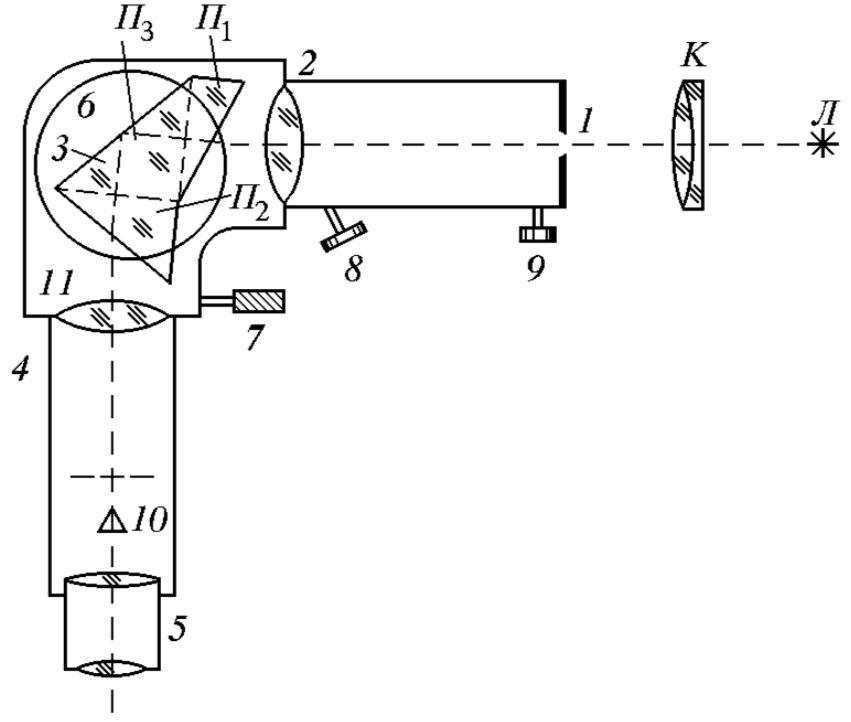
\includegraphics[scale=0.2]{scheme.png}
	\caption{Схема экспериментальной установки}
	\label{fig:scheme}
\end{wrapfigure}
\paragraph{Экспериментальная установка.}
Для измерения длин волн спектральных линий в работе используется стеклянно-призменный монохроматор-спектрометр УМ-2, предназначенный для спектральных исследований в диапазоне от 0.38 до 1.00 мкм.\par
Спектрометр УМ-2 нуждается в предварительной градуировке. Для градуировки в коротковолновой части спектра удобно применять ртутную лампу ПРК-4, а в длинноволоновой и средней --- неоновую лампу.\par
При подготовке УМ-2 к наблюдениям особое внимание следует обращать на тщательную фокусировку, с тем чтобы указатель 10 и спектральные линии имели четкие, ясные границы.\par
Основные элементы монохроматора представлены на рис. \ref{fig:scheme}\par
\begin{enumerate}
	\item Входная щель 1, снабжённая микрометрическим винтом 9, который позволяет открывать щель на нужную ширину (в диапазоне 0.01-4 мм).
	\item Коллиматорный объектив 2, снабженный микрометрическим винтом 8. Винт позволяет смещать объектив относительно щели при фокусировки спектральных линий различных цветов.
	\item Сложная спектральная призма 3, установленная на поворотном столике 6. Призма 3 состоит из 3-х склеенных призм $\text{П}_1$, $\text{П}_2$ и $\text{П}_3$. Первые две призмы с преломляющими углами $30^\circ$ изготовлены из тяжёлого флинта, обладающего большой дисперсией. Промежуточная призма $\text{П}_3$ сделана из крона. Лучи отражаются от её гипотенузной грани и поворачиваются на $90^\circ$. Благодаря такому устройству дисперсия призм $\text{П}_1$ и $\text{П}_2$ складываются.
	\item Поворотный столик 6, вращающийся вокруг вертикальной оси при помощи микрометрического винта 7 с отсчётным барабаном. На барабан нанесена винтовая дорожка с градусными делениями. Вдоль дорожки скользит указатель барабана. При вращении барабана призма поворачивается, и в центре поля зрения появляются различные участки спектра.
	\item Зрительная труба, состоящая из объектива 4 и окуляра 5. Объектив дает изображение входной щели 1 различных цветов в своей фокальной плоскости. В этой же плоскости расположено острие указателя 10. Изображение щели рассматривается через окуляр 5. В случае необходимости окуляр может быть заменен выходной щелью, пропускающей всего одну из линий спектра --- тогда прибор служит монохроматором. В нашей работе выходная щель не применяется, то есть прибор используется как спектрометр.
	\item Массивный корпус 11, предохраняющий прибор от повреждений и загрязнений.
	\item Оптическая скамья, на которой могут перемещаться рейтеры с источником света Л и кондесором К, служащим для концентрации света на входной щели. Входная щель спектрометра, конденсор и источник должны быть на одной высоте. Проходящий через входную щель световой пучок хорошо заполняет конденсор и призму, если выполнено соотношение $D_k/b=D_2/f_2=1/6$, где $D_k$ -- диаметр конденсора, $b$ -- расстояние от конденсора до входной щели, $D_2$ и $f_2$ -- диаметр и фокусное расстояние коллиматорного объектива 2.
\end{enumerate}
\paragraph{Водородная лампа.}
В опытах по изучению длин волн бальмеровской серии источником света служит водородная трубка H-образной формы, питаемая от источника высокого напряжения. Наибольшая яркость спектра достигается в том случае, когда источником света служит торец горизонтальной части трубки -- капилляра (перемычки в букве H).\par
Для увеличения яркости интересующих нас линий атомарного водорода в состав газа, которым заполняют трубку при её изготовлении, добавляют пары воды. Молекулы воды в электрическом разряде разлагаются, образуя атомарный водород. Трубка заполняется газом до давления 5--10 Торр.\par
Следует отметить, что в спектре водородной лампы наряду с линиями атомного спектра наблюдается также спектр молекулярного водорода. Однако интенсивность молекулярных линий значительно слабее и отождествление ярких атомных линий на фоне молекулярного спектра не представляет большого труда.
\section{Ход работы}
\begin{enumerate}
	\item Проведем градуировку монохроматора. График для зависимости длины волны $\lambda$ от номера пикселя в матрице фотоаппарата приведен на рис. \ref{fig:calibration}. В таблице \ref{table:calapprox} приведены параметры аппроксимации функции $\lambda(N)$ по формуле
	\begin{equation}
		\lambda=A+\frac{C}{N-B}
	\end{equation}
	\begin{figure}[h]
			\begin{tikzpicture}
				\begin{axis}[
					title={$\lambda=f\left(N\right)$},
					xlabel={$N$},
					ylabel={$\lambda\ \angstrom$.},
					xmin=700,
					xmax=2200,
					ymin=4800,
					ymax=6300,
					ymajorgrids=true,
    				xmajorgrids=true,
    				grid style=dashed,
    				width=\textwidth,
				]
				\addplot+[
					color=black,
    				mark=square,
    				only marks,
					error bars/.cd,
					y dir=both, y explicit,
					x dir=both, x explicit
				]
				coordinates{
					(703.93, 4916.04)+-(0.815763,0)
					(780.374, 4960.32)+-(1.55008,0)
					(888.13, 5025.64)+-(1.40821,0)
					(920.305, 5045.82)+-(1.55534,0)
					(1037.08, 5121.55)+-(1.50279,0)
					(1306.8, 5316.69)+-(1.16125,0)
					(1356.52, 5354.05)+-(1.67356,0)
					(1369.4, 5365.06)+-(1.63941,0)
					(1394.32, 5384.7)+-(1.15862,0)
					(1485.18, 5460.74)+-(2.20296,0)
					(1719.21, 5675.86)+-(1.37143,0)
					(1812.27, 5769.59)+-(2.93727,0)
					(1832.35, 5790.65)+-(3.55205,0)
					(1844.65, 5803.65)+-(1.22956,0)
					(1896.44, 5859.38)+-(1.02857,0)
					(1907.94, 5872.03)+-(1.38325,0)
					(1923.83, 5888.94)+-(1.20591,0)
					(2077.89, 6072.64)+-(1.60525,0)
					(2118.27, 6123.27)+-(1.35829,0)
					(2202.11, 6234.37)+-(1.48177,0)
				};
				\addplot[
					domain=700:2200,
					samples=200,
					color=black
				]
				{2510.01+((-1.01864*10^7)/(x - 4937.46))};
				\end{axis}
			\end{tikzpicture}
			\caption{Зависимость $\lambda=f(N)$}
			\label{fig:calibration}
		\end{figure}
		\begin{table}[!h]
			\centering
			\caption{Параметры аппроксимации}
			\begin{tabular}{|c|c|}
				\hline
				Параметр & Значение\\
				\hline
				A & $2510.01 \pm 0.39$\\
				B & $4937.46 \pm 0.42$\\
				C & $(-1.01864 \pm 0.00014)\cdot10^7$\\
				\hline
			\end{tabular}
			\label{table:calapprox}
		\end{table}
		\item Измерим спектр водородной лампы и попытаемся определить положение линий $H_{\alpha}$, $H_{\beta}$, $H_{\gamma}$ и $H_{\delta}$. Черными точками на графике зависимости интенсивности от длинны волны обозначены указанные в таблице \ref{table:peaks} линии спектра.
		\begin{figure}
		    \minipage{1\textwidth}
		    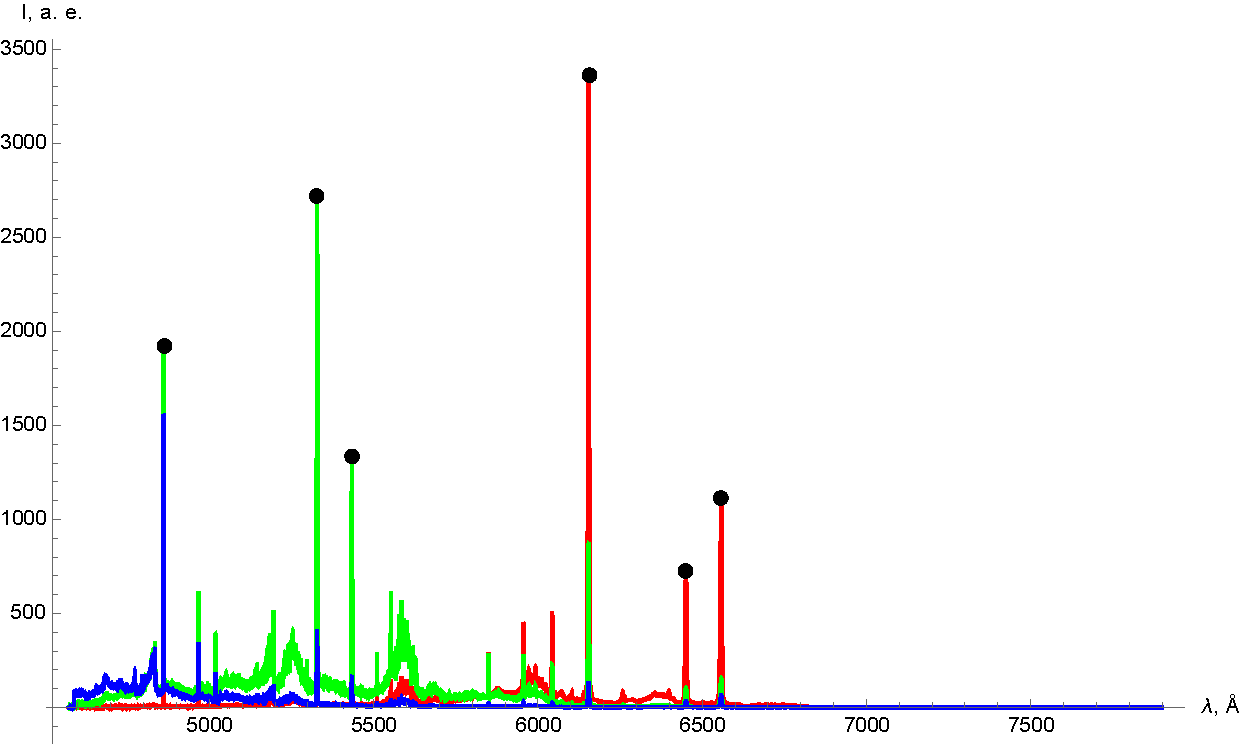
\includegraphics[width=\linewidth]{h2_plot_peaks.pdf}
		    \endminipage\\
		    \minipage{1\textwidth}
		    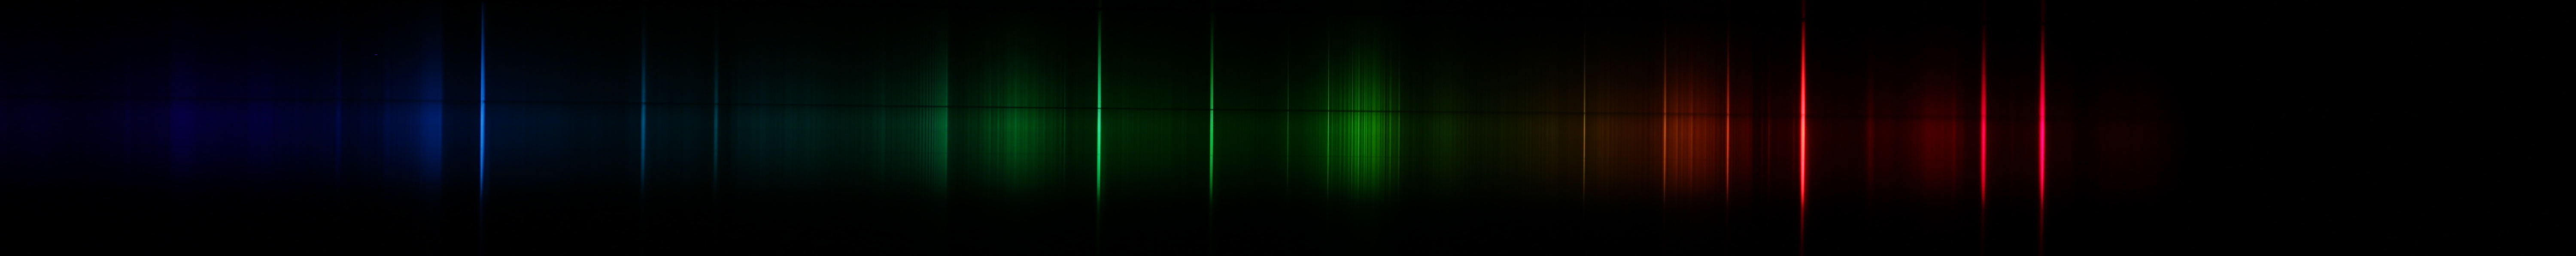
\includegraphics[width=\linewidth]{h2_spectre.JPG}
		    \endminipage
		    \caption{График зависимости интенсивности от длинны волны в спектре водорода и фотография полученного спектра водорода}
		\end{figure}
		\begin{table}
		    \centering
		    \caption{Полученные линии спектра водорода}
		    \begin{tabular}{|c|c|c|c|c|c|c|}
		        \hline
		        № & 1 & 2 & 3 & 4 & 5 & 6\\
		        \hline
		        $\lambda,\ \angstrom$ & 4860.5 & 5328.18 & 5434.16 & 6154.2 & 6450.97 & 6557.78 \\
                $I,\ a.e.$ & 1918.2 & 2716.69 & 1335.84 & 3363.92 & 729.517 & 1112.86 \\
                \hline
		    \end{tabular}
		    \label{table:peaks}
		\end{table}
		Сравним полученные линии спектра с линиями в серии Бальмера, приведенными в таблице \ref{table:balmer}.
		\begin{table}[]
		    \centering
		    \caption{Серия Бальмера}
		    \begin{tabular}{|c|c|c|c|c|}
		        \hline
		        $H_{\alpha}$ & $H_{\beta}$ & $H_{\gamma}$ & $H_{\delta}$\\
		        \hline
		         6563 $\angstrom$ & 4861 $\angstrom$ & 4340 $\angstrom$ & 4102 $\angstrom$\\
		         \hline
		    \end{tabular}
		    \label{table:balmer}
		\end{table}\par
		Видно, что линия 6 ($6557.78\angstrom$) близка по величине к $H_{\alpha}$, а линия 1 ($4860.5\angstrom$) близка к $H_{\beta}$. Остальные линии серии Бальмера не вошли в полученный спектр. Однако в изображении присутствуют и другие линии (2-5). Вероятнее всего они принадлежат атомарному кислороду, образовавшемуся из водяных паров, присутствующих в лампе.
\end{enumerate}
\end{document}
